% Implementation: Umsetzung, Probleme, Lösungen
\chapter{Implementierung}\label{chap::impl}
Das Implementierungskapitel enthält eine genauere Beschreibung der Implementierung der Arbeitspakete aus Abschnitt \ref{sec::workpacks}.
Die Beschreibungen sollen einen Überblick geben, wie die Arbeitspakete umgesetzt wurden ohne zu stark ins Detail zu gehen.

\section{Strukturelle Modifikationen}\label{sec::sm}
Das Projekt wurde strukturell modifiziert und für die Integration der Arbeitspakete vorbereitet.
So wurde im Volumerenderwidget eine globale Variable erstellt, welche den Wert der aktuellen Raycast Methode beinhaltet.
In der paintGL() Methode wurde dann über diese Variable in einem switch-case die jeweilige Methode aufgerufen, die die Berechnung des aktuellen Raycasts durchführt.
Da die Raycasts durch einen OpenCL Kernel berechnet werden und nicht direkt gerendert werden, werden die Ergebnisse immer in einer Textur abgespeichert, welche durch OpenGL auf ein Fullscreen-Quad gezeichnet wird.
Da die MDC Methode zwei verschiedene Texturen verwendet, wurde dementsprechend der Fragment-Shader durch ein switch-case ergänzt, welches für jede Raycast Methode unterschiedliche Anweisungen ausführen kann.

Die Kernfunktion des Raycasts, die Strahlverfolgung, bleibt für alle Raycast Methoden die gleiche.
Daher wurde dieses Prinzip im OpenCL Kernel auch angewandt.
Ein switch-case, relativ am Anfang des Raycast Kernels, führt je nach aktueller Raycast Methode die entsprechenden Operationen aus.
Dadurch konnte für alle Raycast Methoden der gleiche Raycast Kernel verwendet werden, welcher lediglich mit unterschiedlichen Parametern ausgeführt wurde.

Die GUI des Projekts wurde mit einigen Funktionen ergänzt über die bestimmte Parameter verändert werden konnten.
Dies ermöglichte insbesondere die einfache Umstellung der Raycast Methoden zur Laufzeit des Projekts.

\section{Implementierung der Arbeitspakte}\label{sec::ida}
Im folgenden werden die genaueren Umsetzungen der Arbeitspakete vorgestellt, insbesondere die Implementierung des MDC und DDC Raycasts sowie die Anpassung der Strahlabtastrate.
Zusätzlich wird beschrieben, wie die Messungen im Projekt vorbereitet wurden, so dass Messwerte erstellt werden konnten.

\subsection{Simulieren der Blickposition}\label{sec::ida::sdb}
Da die Einbindung des Eyetrackers für das oberflächliche Testen der Raycast Methoden nicht notwendig ist, wurde die Blickposition vorerst mit der Mausposition simuliert.
Das Volumerenderwidget verfügt über eine Callback-Methode, die auf Mausbewegungen reagiert.
Diese Methoden wurde sich zu Nutze gemacht, so dass durch einen Aufruf dieser Methode, aufgrund einer Veränderung in der Mausposition, sofort die aktuelle Position des Mauszeigers bezüglich des Volumerenderwidgets in einer globalen Variable abgespeichert wurde.
Damit jede Raycast Methode diese auch zu Verfügung hat, wurde diese zu Beginn der paintGL() Methode dem OpenCL Raycast Kernel übergeben. (Arbeitspaket aus Abschnitt \ref{sec::workpacks::sdb})

\subsection{Reduzierung der Strahlabtastrate im peripheren Bereich}\label{sec::ida::rdsifb}
Die Reduzierung der Strahlabtastrate wurde im Raycast Kernel implementiert.
Nachdem alle Operationen der jeweiligen Raycastmodifikationen ausgeführt wurden, wurde für jedes Work-Item die Distanz der zugehörigen Bildkoordinate des entsprechenden Strahls zu der Mausposition berechnet.
Im MDC Raycast lag die Bildkoordinate nur normalisiert vor und wurde dementsprechend vor der Distanzberechnung umgerechnet.

Sei nun $\vec{r}$ ein 2D-Vektor, der die x- und y-Position der Bildkoordinate eines Strahls enthält und $\vec{m}$ ein 2D-Vektor, der die Bildkoordinaten der Mausposition enthält.
Die Distanz zwischen der Mausposition und einem Strahl wurde wie folgt berechnet: $d = \texttt{length(}\vec{r}-\vec{m}\texttt{)}$.
Die Funktion \texttt{length()} ist eine \emph{Built-In OpenCL Function} und berechnet die Länge eines Vektors.
Mit der Distanz $d$ zwischen einem Strahl und der Mausposition wurde ein Faktor $sf$ berechnet: $sf = 1,0 - d  / ib$.
Hierbei bezeichnet $ib$ die maximale Distanz zwischen zwei Bildkoordinaten, also die Länge der Diagonale des Bildes.
Ist $d < 10$ wird die Strahlabtastrate $sr$ nicht verändert.
Ansonsten berechnet sich die neue Strahlabtastrate mit $sr = \texttt{max(}sf * sr,\,t\texttt{)}$, wobei die Funktion \texttt{max()} auch eine \emph{OpenCL Built-In Function} ist.
Bei einer zu geringen Abtastrate kann es vorkommen, dass vor allem dünne Strukturen eines Volumens von einigen Strahlen gar nicht oder nur sehr geringfügig abgetastet werden und es so sich kleine bis große Löcher in diesen Flächen bilden können.
$t = 0,25$ hat sich als guter Schwellwert erwiesen, der auch bei großen Distanzen zwischen einem Strahl und der Mausposition kaum Artefakte generiert. (Arbeitspaket aus Abschnitt \ref{sec::workpacks::ors})

\subsection{Reduzierung der Strahldichte im peripheren Bereich}
Die Reduzierung der Strahldichte im peripheren Bereich wurde durch zwei verschiedene Methoden umgesetzt, die MDC Methode (Abschnitt \ref{ss::MDC}) und die DDC Methode (Abschnitt \ref{ss::DDC}).
Im folgenden werden die Implementierungen beider Methoden getrennt voneinander beschrieben.

\subsection{MDC Implementierung}
\begin{figure}[]
	\centering
	\begin{minipage}[t]{0.49\textwidth}
		\centering
		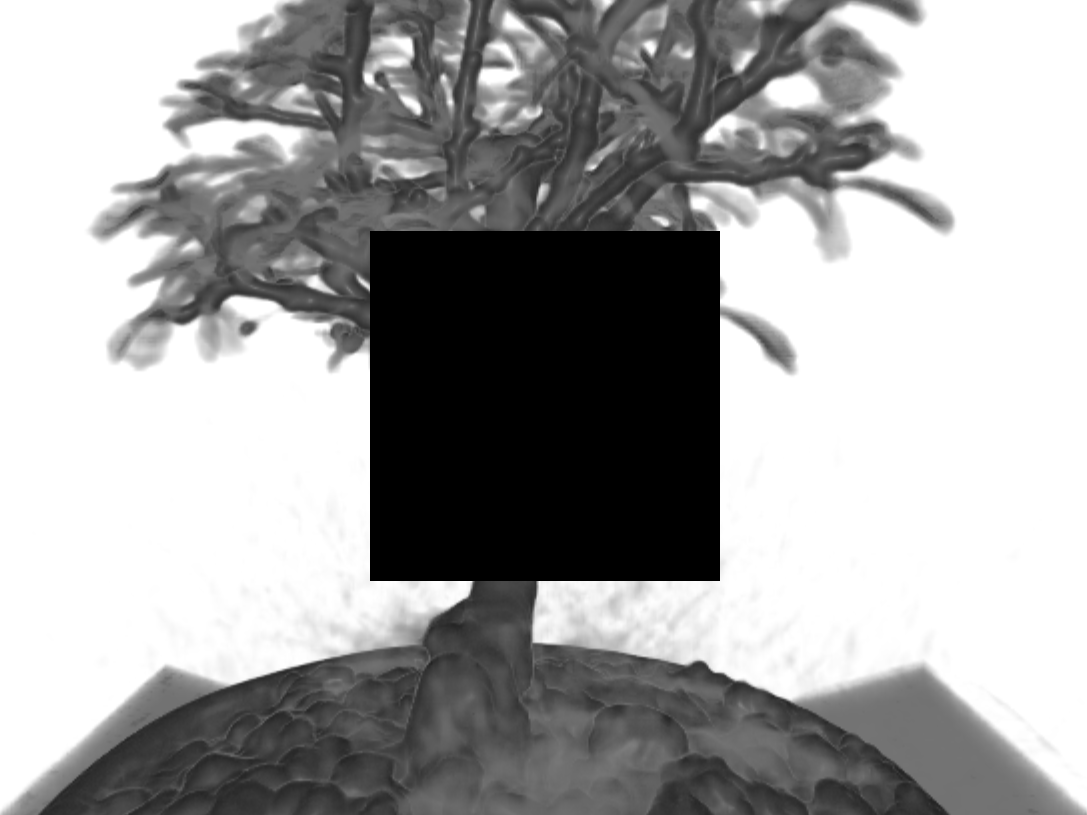
\includegraphics[width=1\textwidth]{../../Grafiken/results/implementierung/mdc_ol.png}
		\caption{Ausschnitt einer Berechnung mit dem MDC Raycast, bei der nur der äußere niedrig aufgelöste Bereich angezeigt wird. Der niedriger aufgelöste Bereich hat nur ein Viertel der normalen Auflösung.}
		\label{fig::imp::mdc_ol}
	\end{minipage}
	\hfill
	\begin{minipage}[t]{0.49\textwidth}
		\centering
		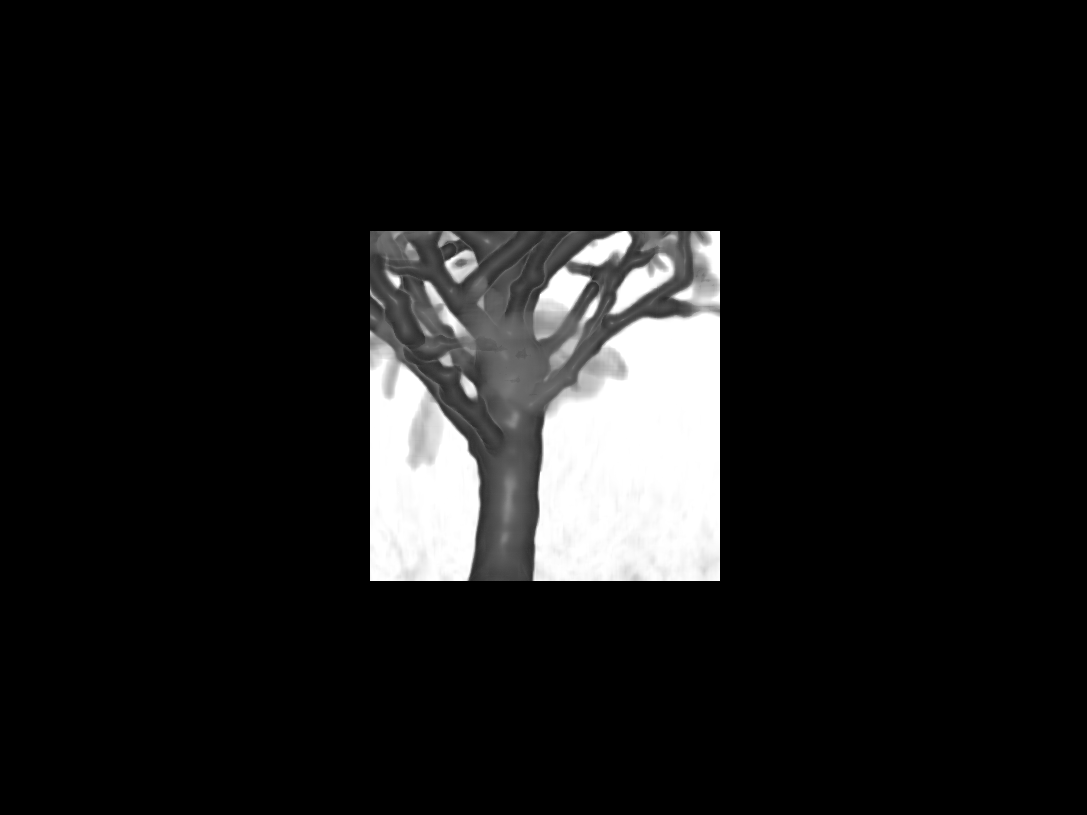
\includegraphics[width=1\textwidth]{../../Grafiken/results/implementierung/mdc_il.png}
		\caption{Ausschnitt einer Berechnung mit dem MDC Raycast, bei der nur der innere, normal aufgelöste Bereich angezeigt wird.}
		\label{fig::imp::mdc_il}
	\end{minipage}
\end{figure}

Die Implementierung des MDC Raycasts wurde in einer eigenen Methode des Volumerenderwidgets umgesetzt, die von der paintGL() Methode aufgerufen wird.
Für die Berechnung des Raycasts konnte die bisherigen Funktionen des \texttt{volumerendercl} Objektes wieder verwendet werden und wurde zwei Mal hintereinander ausgeführt.
Zuerst wurde der Kernel mit einer in x- und y-Richtung halbierter Anzahl an Work-Items gestartet.
Da ein Work-Item einen Pixel berechnet, wurde dadurch das Bild in nur einem Viertel der ursprünglichen Auflösung berechnet.
Daher wurde für die Ausgabe des Raycasts hier eine neue Textur verwendet, deren Größe ebenfalls nur ein Viertel der ursprünglichen Auflösung ist.
In dem jeweiligen Teil des switch-case im Rayast Kernel, der beim MDC Raycast ausgeführt wird, konnte über einen Parameter entschieden werden, ob es die erste oder die zweite Ausführung des Raycasts Kernels innerhalb der MDC Methode ist.
Ist es der erste Aufruf, so wurden innerhalb eines festgelegten Quadrats um den Mauszeiger herum alle in diesem Quadrat sich befindenden Work-Items zu Beginn des Kernels discarded.
Die Ausmaße des Quadrat wurden dem Kernel als Parameter übergeben.
Anschließend führte der Raycast Kernel den normalen Ablauf fort.
Wurde nun die berechnete Textur auf das OpenGL Fullscreen-Quad projiziert, so sah das berechnete Bild ungefähr so aus, wie es in Abbildung \ref{fig::imp::mdc_ol} dargestellt ist.
Der äußere Bereich des Bildes hat hier also nur ein Viertel der normalen Auflösung.
Die Interpolation dieser niedrigen Auflösung auf die normale wurde dabei durch den OpenGL Fragment Shader beim Auslesen der Texturdaten geregelt.
Der innere Bereich des Bildes entspricht den Work-Items, die frühzeitig im Raycast Kernel discarded wurden, wodurch die Textur an dieser Stelle schwarz ist.
Bei der zweiten Ausführung wurde der Kernel mit der normalen Anzahl an Work-Items gestartet.
Dafür wurde eine andere Textur verwendet, deren Größe der normalen Auflösung entspricht.
Im Gegensatz zur ersten Ausführung wurde nun der äußere Bereich, also alle Work-Items, die sich außerhalb des Quadrat befanden, discarded.
Entsprechend sah das Ergebnis dieser Ausführung in etwa so aus, wie in Abbildung \ref{fig::imp::mdc_il}.
Hier wurde aber die Größe des Quadrats durch einen Offset ergänzt, wodurch bei der Zusammenfügung der Bilder keine schwarze Umrandung des Quadrat übrig bleibt.

Bei der Implementierung mussten beachtet werden, dass aufgrund dessen, das bei den verschiedenen Ausführungen verschieden Viele Work-Items gestartet wurden, die ID's der Work-Items nicht immer mit ihrer zugehörigen Bildkoordinate übereingestimmt haben.
Daher wurden alle Werte, die sich auf Bildpositionen beziehen, normalisiert.
Wie zum Beispiel die Mausposition und die Ausmaße des Rechtecks, welche schon im Host-Code der paintGL() Methode normalisiert wurden, sowie die IDs der Work-Items im Kernel.

Das Zusammenfügen der Bilder wurde im OpenGL Fragment Shader durchgeführt.
Der Fragment Shader hat dafür die selben Parameter übergeben bekommen, wie der OpenCL Kernel.
Eine normalisierte Texturkoordinate wurde dann wie eine normalisierte Work-Item ID behandelt und je nach dem ob sich die Texturkoordinate innerhalb des Quadrats befunden hat oder nicht, wurde der Farbwert in der entsprechenden Textur ausgelesen.

\subsection{DDC Implementierung}
\begin{figure}[]
	\centering
	\begin{minipage}[t]{0.49\textwidth}
		\centering
		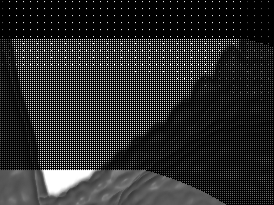
\includegraphics[width=1\textwidth]{../../Grafiken/results/implementierung/ddc_o_ip_cut.png}
		\caption{Ausschnitt einer Berechnung mit dem DDC Raycast.}
		\label{fig::imp::ddc_o_ip}
	\end{minipage}
	\hfill
	\begin{minipage}[t]{0.49\textwidth}
		\centering
		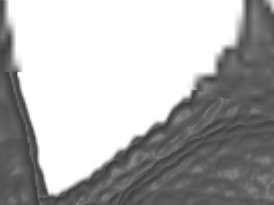
\includegraphics[width=1\textwidth]{../../Grafiken/results/implementierung/ddc_m_ip_cut.png}
		\caption{Ausschnitt einer Berechnung mit dem DDC Raycast.}
		\label{fig::imp::ddc_m_ip}
	\end{minipage}
\end{figure}
Der DDC Raycast ist die Implementierung des Arbeitspakets in Abschnitt \ref{ss::DDC}.
Wie für die Implementierung des MDC Raycasts wurde dafür eine eigene Methode geschrieben, die von der paintGL() Methode aufgerufen wird.
Auch hier wurden die Funktionen des \texttt{volumerendercl} Objektes wiederverwendet und der Raycast über dieses Objekt gestartet.
Anders als im ursprünglichen Raycast und MDC Raycast steht der Index eines Work-Items nicht mehr im direkten Zusammenhang mit einer Bildkoordinate, sondern die IDs wurden durch eine Funktion auf ganz unterschiedliche Bildkoordinaten zugewiesen.
Daher war die Wahl des Verhältnisses der Anzahl der Work-Items in x- und y-Richtung nicht mehr wichtig, sondern ausschlaggebend war wie viele Work-Items insgesamt gestartet wurden.

Die DDC Methode sollte drei Bereiche berechnen, die im Anschluss interpoliert werden.
Der äußerste Bereich sollte die niedrigste Auflösung haben.
Der mittlere Bereich sollte eine dazwischenliegende und der innere Bereich die normale Auflösung besitzen.
Der mittlere und innere Bereich sollen dabei durch Ellipsen beschränkt werden und ihr Mittelpunkt liegt auf der Mausposition.
Die Auflösung des mittleren Bereichs und des äußeren Bereichs wurde dafür mit einem Wert angegeben, der die $Anzahl der Texel - 1$ angibt, die je zwei Strahlen in x- und y-Richtung voneinander entfernt sind.
Dieser wert wurde \emph{G-Wert} genannt.
Ein G-Wert von $1$ würde bedeuten, dass zwei Strahlen ein Texel voneinander entfernt sind.
Also zwischen ihnen keine Lücke besteht.
Das heißt, ein G-Wert von $1$ entspricht der normalen Auflösung.

Die G-Werte der unterschiedlichen Bereiche wurde vor dem Start des Raycasts festgelegt, da diese notwendig sind, um die benötigte Anzahl an Work-Items zu bestimmen.
Um die Anzahl der insgesamt benötigten Work-Items abzuschätzen, wurden die Ellipsen als Rechtecke betrachtet.
Für die drei Bereiche ergab sich die abgeschätzte Anzahl benötigter Work-Items dann aus $\frac{AnzahlDerPixelDesBereichs}{GWertDesBereichs}$.
Für jeden Bereich wurde diese Anzahl anschließend mit einem geringen Offset erhöht, damit später keine Work-Items fehlen.
Die Anzahl der Work-Items der Bereiche wurde zusätzlich ohne den Offset dem Raycast Kernel als Parameter übergeben.
Die Summe dieser Werte ergab die abgeschätzte gesamte Anzahl an Work-Items, mit welcher der Raycast Kernel gestartet wurde.

Im Raycast Kernel wurden die zweidimensionalen globalen IDs der Work-Items auf eine eindeutige eindimensionale ID abgebildet.
Diese waren dem Bereich von $0$ bis zur maximalen Anzahl an $gestarteteWorkItems-1$ zugeordnet.
Ist $m$ die Größe der x-Dimension des Kernels und $xId$ und $yId$ die globale ID des Work-Items, so berechnete sich die neue ID mit: $nId = yId * m + xId$.
Mit der neuen ID $nId$ und den übergebenen Werten für die maximale Anzahl der Work-Items in den unterschiedlichen Bereichen konnte für jedes Work-Item festgelegt werden, welchem Bereich es zugeordnet werden soll.
Da nun der Bereich in welchem sich ein Work-Item befindet, bekannt war, konnte für dieses Work-Item der G-Wert $g$ sowie die ursprüngliche Bereite des Bereiches $m$ bestimmt werden.
Das heißt für ein Work-Item, welches im inneren Bereich liegt, galt $g=1$ und $m=BreiteDerInnerenEllipse$.
Ein Work-Item welches im äußeren Bereich lag, hat einen höheren G-Wert zugewiesen bekommen und für $m$ die Breite der Ausgangstextur.
Für die Messungen im Abschnitt \ref{chap::resdisc} wurde für den äußeren Bereich ein G-Wert von $7$ und für den mittleren Bereich ein G-Wert von $2$ verwendet.
Mithilfe der bekannten Werte $m$ und $g$ sowie dem Wissen, wie viele Work-Items den unterschiedlichen Bereichen zugeorndet wurden, wurde die $nId$ mit ein paar kleinen Anpassungen wieder zurück in eine zweidimensionale ID überführt, die nun einer Bildkoordinate entspricht.
Mit der neuen Work-Item ID kann ein Work-Item die Berechnung eines Strahls, wie bei dem ursprünglichen Raycast ganz normal fortsetzen.
Abbildung \ref{fig::imp::ddc_o_ip} zeigt einen Ausschnitt der berechneten Textur des DDC Raycasts ohne eine anschließende Interpolation der Werte.
Man kann erkennen, dass im äußeren Bereich der Abstand zwischen den Strahlen deutlich größer ist, als in dem mittleren und inneren Bereich.
Man sieht auch, dass die unterschiedlichen Bereiche sich gegenseitig überlappen.
Dies ist für die anschließende Interpolation notwendig, da sonst zwischen den Bereichen schwarze Punkte entstehen können.

Abbildung \ref{fig::imp::ddc_m_ip} zeigt das in Abbildung \ref{fig::imp::ddc_o_ip} dargestellte Bild nachdem es interpoliert wurde.
Die Interpolation wurde für den DDC Raycast in einem eigenen Kernel implementiert und nicht wie beim MDC Raycast durch den Fragmentshader realisiert.
Der Kernel für die Interpolation der Werte wurde für die gesamte Auflösung des Bildes gestartet.
Ähnlich wie beim DDC Raycast bestimmt jedes Work-Item den Bereich, in welchem es sich befindet.
Dafür ist es hier nicht notwendig, die Indize umzurechnen, da die IDs der Work-Items schon Bildkoordinaten entsprechen und die Mausposition sowie die Ausmaße der Ellipsen dem Kernel übergeben werden.
Mit der Information, in welchem Bereich sich ein Work-Item befindet und welche G-Werte und Ausmaße die unterschiedlichen Bereiche haben, wurden für ein Work-Item vier umliegende Werte des zuvor berechneten Raycasts ausfindig gemacht und bipolar interpoliert.
Die Ausgabetextur der Interpolation wird durch den Fragmentshader anschließend auf das Full-Screen Quad gezeichnet.

\section{Erstellen und Darstellen von Messwerten}
Für die Umsetzung des Arbeitspakets aus Abschnitt \ref{sec::workpacks::evm}, wurde eine Klasse erstellt, welche für eine Berechnung eines Bildes verschiedene Messwerte speichert.
Diese sind unter Anderem die gesamte Ausführungszeit des Kernels (bei mehreren Ausführungen innerhalb einer Methode wurden diese addiert), die Ausführungszeit der paintGL() Methode und die Mausposition, die in der letzten Ausführung der paintGL() Methode für die Berechnung des Bildes verwendet wurde.
Für jeden Aufruf der \texttt{paintGL()} Methode wurde ein solches Objekt erstellt und gespeichert.
Die letzte Ausführungszeit eines Kernels konnte mit Hilfe des \texttt{volumerendercl} Objektes berechnet werden kann, welches dafür \emph{OpenCL Profiling} Methoden verwendet hat.
Die ungefähre Ausführungszeit der \texttt{paintGL()} Methode selbst wurde mit Hilfe eines \emph{Qt QTime} Objektes berechnet.

Um eine Mausbewegung abzuspeichern wurden globale Variablen erstellt, die den aktuellen Zustand des Volumerenderwidgets bezüglich der Messungen angeben.
Über Tastatureingaben können diese Variablen verändert werden.
Wurde in den Zustand für die Aufzeichnung einer Mausbewegung gewechselt, so hat die Callback-Methode für die Mausbewegungen nicht nur die aktuelle Position in eine globale Variable geschrieben, sondern auch in einen c++ Vektor abgespeichert.
Dies passierte aber nur, falls die zuletzt gespeicherte Position sich um mindestens 10 Pixel von der aktuellen gemessenen Position unterscheidet.
Während Mausbewegungen aufgenommen wurden, wurden die Ausführung der Raycasts blockiert.
Nachdem eine Mausbewegung aufgenommen wurde, konnten die gesammelten Daten gespeichert und wieder geladen.
Falls es eine gespeicherte Mausbewegung gab, konnte über eine Tastatureingabe in den Replay-Zustand gewechselt werden.
In diesem Zustand wurden alle Tastatur- und Mauseingaben bis auf eine Taste, um das Replay vorzeitig abzubrechen, ignoriert.
Wurde in den Replay-Zustand gewechselt, wurde die paintGL() Methode für jede gespeicherte Mausposition in dem c++ Vektor einmal ausgeführt und die dabei gesammelten Messwerte in lesbarer Form in eine \texttt{.txt}-Datei geschrieben.

Mit Hilfe eines Python Scripts konnten die gespeicherten Messwerte geladen und verwertet werden.
Für die Erstellung der Heatmaps und Boxplots wurde \emph{pyplot} aus der Python Bibliothek \emph{matplotlib} verwendet.